\documentclass[10pt,a4paper]{article}
\usepackage[latin1]{inputenc}
\usepackage{amsmath}
\usepackage{amsfonts}
\usepackage{amssymb}
\usepackage{graphicx}
\usepackage{float}
\author{Michele De Vita}
\begin{document}
	\begin{enumerate}
		\item  
		\begin{align*}
	 &i) \,\,\, \mathbf{C} = (0,  5, -7, 0), &d = -2  \\
		& ii) \,\,\, \mathbf{C} = \left( \begin{matrix}
		0 & 1 & -1 & 0 & 0 \\ 
		0 & 0 & 1 & -1 & 0 
		\end{matrix} \right) ,  &d= \left( \begin{matrix}
		0 \\ 
		0
		\end{matrix} \right)
		\end{align*}
		\item 
		This plot shows the SSE in function of $ \beta $:
		\begin{figure}[H]
			\centering
			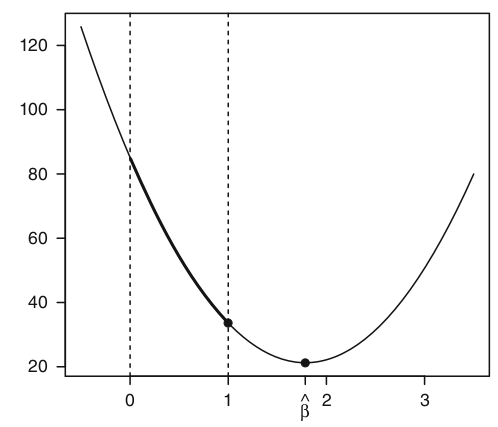
\includegraphics[width=0.7\linewidth]{plot_ftest}
		\end{figure}
		The F-test score is $ \dfrac{SSE_{H_0} - SSE}{SSE} $ where $ SSE = SSE(\hat{\beta}) $ that is the y in the plot where $ x = \hat{\beta} $ and $ SSE_{H_0} = SSE(\beta = 1) $\\
		The plot for the numerator of Wald test is the same of the previous because the numerator is the same except for a square difference instead of normal difference.\\
		The main difference between F-test and Wald test is the denominator in the first is $ \hat{\theta} $ while in the second is $ var(\hat{\theta}) $. There is also a relation between test statistics $ F $ and $ W $: $ W = rF $
		\item The confidence interval for $ \mu_0  $ is $ \mathbf{x}_0' \hat{\beta} \pm t_{n-p}(1-\alpha / 2) \hat{\sigma} (\mathbf{x}_0' (\mathbf{X'X})^{-1} x_0)^{1/2}$ while for prediction is $ \mathbf{x}_0' \hat{\beta} \pm t_{n-p}(1-\alpha / 2) \hat{\sigma} (1 + \mathbf{x}_0' (\mathbf{X'X})^{-1} x_0)^{1/2}$. The difference between the two formulas is the "$ 1\,\,+ $" near $ x_0 $ that become from the fact that the estimation try to give an confidence interval of a parameter , so with no variance, while the prediction try to estimate a aleatory variable with a expected value and a variance.
		\item $ f(x_0) = \mathbf{x}_0' \hat{\beta} \pm t_{n-2}(1-\alpha / 2) \hat{\sigma} (1 + \mathbf{x}_0' (\mathbf{X'X})^{-1} x_0)^{1/2}$
		where $ X = $
		$ \left( \begin{matrix}
			1 & x_{11} \\ 
			\vdots & \vdots  \\ 
		1 & x_{n1}
			\end{matrix} \right)$ and $ p = 2 $.\\
			The length of interval is minimum when $ \mathbf{x_0 = \mu}  $ because we can write the product $ \mathbf{x_0'(X'X)^{-1}x_0}  $ as $ \dfrac{\sum(x_i - x_0)^2}{dev(x)} $ then the numerator $  \sum(x_i - x_0)^2 $ is minimized when $ x_0 = \mu $
			\item Increasing the number of parameters is not always a good idea: we can express the SPSE (expected squared prediction error as):
			$ \underbrace{n\sigma^2}_{irreducible\,\,  part} + \underbrace{|M|\sigma^2}_{Variance \,\, error} + \underbrace{\sum_{i=1}^{n} (u_{i M} - u_i)^2}_{BIAS^2} $
			\item If we consider only $ \mathbf{X_1} $ we have $ \mathbf{X = X_1} $ then 
			\begin{align*}
				E\left[ \tilde{\beta}_1 \right]		&= E \left[ \mathbf{(X_1'X_1)^{-1} X_1'y} \right] \\
				&=  \mathbf{(X_1'X_1)^{-1} X_1' } E \left[ \mathbf{y} \right] \\
				&=  \mathbf{(X_1'X_1)^{-1} X_1' (X_1 \beta_1 + X_2 \beta_2)} \\
				&= \beta_1 +\mathbf{(X_1'X_1)^{-1} X_1'  X_2 \beta_2}
			\end{align*}
			The bias vanish if $ \mathbf{X_1'  X_2  = 0} $ that in statical words mean that $ \mathbf{X_1} \text{ and } \mathbf{X_2} $ are uncorrelated or when $ \mathbf{\beta_2}  $ is irrelevant
			\item If we omit a relevant covariate, we can have a decrease the variance of model such that the increase of $ bias^2 $ is overall convenient
			\item $ SPSE = \sum (y_{n+i} - \hat{y}_{iM}^2) $. See point 5
			\item 
			\begin{align*}
			E\left( SSE \right) &= E\left( \sum \left( y_i - \hat{y}_{iM} \right)^2 \right)  \\
			&= E \left( \mathbf{\varepsilon' \varepsilon} \right) \\
			&= (n-p) \sigma^2 \\
			&= E(SPSE) - 2  |M|\sigma^2 \\
			&= n \sigma^2 + |M|\sigma^2 -2 |M|\sigma^2 \\
			&= n \sigma^2 - |M|\sigma^2 \\
			&= (n-p)\sigma^2
			\end{align*} 
			$ SSE $  underestimate the $ SPSE $ because $ \hat{SPSE} = \hat{SSE} + 2  |M| \hat{\sigma}^2$ .\\
			This bias is more severe for complex models because the bias is proportional to model complexity
			\item $ AIC =n \log(\hat{\sigma}^2) + 2 (|M| + 1) $\\
			$ BIC = n \log(\hat{\sigma}^2) + \log(n) (|M| + 1) $.\\
			Since $ SPSE  $ is not observable the two latter indicators are used to evaluate the fit of the model.\\
			The difference between $ AIC \text{ and } BIC $ is the term before $ (|M| + 1) $: in AIC is equal to 2 while in BIC is $ \log(n) $. This mean that BIC have a major penalty when the model complexity increase in big dataset.\\
			For $ n = 100 $ we have for $ l = -300, |M| = 5 $ $ AIC = 612, \,\, BIC = 627.63 $ while with $ l = -290, |M| = 9 $ $ AIC = 600, BIC = 626.05 $.\\
			For $ n = 200 $ we have the same $ AIC $ while $ BIC $ changes with parameters $ l = -300, |M| = 5 $  we have $ BIC = 631.79 $ and with  $ l = -290, |M| = 9 $ $ BIC = 632.98 $.
			Between $ n = 100 $ and $ n = 200 $ we can note the phenomenon described before with BIC, because with $ n = 100 $ there is a decrement of BIC between the two configurations while for $ n = 200 $ the BIC increase between the two configurations
			\item $ VIF_j = \dfrac{1}{1 - R_j^2} $.\\It measures the correlation between the covariate $ x_j $ with the other covariates. The greater is $ R^2_j \in [0,1]$ the greater is $ VIF_j $. An empiric alert for variance is when $ VIF_j > 10 $
			\item The ridge regression add a penalty term $ \lambda $ to the linear regression. The $ \mathbf{PLS(\beta) = (y - X \beta)'(y - X \beta) + \lambda \beta' \beta} $.\\The ridge regression is biased respect to linear regression:\\
			$ E_{LS}(\hat{\beta}) = \mathbf{(X'X)^{-1} X'X \beta = \beta} $\\
			$   E_{PLS}(\hat{\beta}) = \mathbf{(X'X + \lambda X'X)^{-1} X'X \beta} $   (when penalty = 0 $  E_{PLS}(\hat{\beta}) = E_{LS}(\hat{\beta})   $)\\
			When $ \lambda $ increases the coefficients $\beta $ tends to zero because $ \mathbf{\lambda K = (X'X + \lambda K)- X'X} $. If we multiply two definite semipositive matrices $ \mathbf{(X'X + \lambda K)^{-1}} $ with $  \mathbf{(X'X + \lambda K)- X'X}  $ also the result is definite semipositive  that is $ \mathbf{I_p - (X'X + \lambda K)^{-1}X'X}  $. This imply that $ \mathbf{(X'X + \lambda K)^{-1}X'X}    $ have the diagonal elements between $[0,1] $ and this term appears when we express $ \hat{\beta}_{PLS} $ in function of $ \hat{\beta}_{LS} $:\\
			$ \hat{\beta}_{PLS} =  \mathbf{(X'X + \lambda K)^{-1}X'X \beta_{LS}}   $\\
			The covariance matrix of $ \hat{\beta}_{PLS} $ for the same reason is lower than variance of $ \hat{\beta}_{LS} $ so in some cases can be convenient use a ridge regression when the bias error is less relevant than variance error 
	\end{enumerate}
\end{document}